
% Auto-generated from suite_20260404T090445Z_factorial
\section{Quantitative Results}
The balanced full-factorial suite comprised 600 completed runs ($4$ engines $\times$ $3$ models $\times$ $5$ prompts $\times$ $10$ replicates).
The analysis below is based on the final output of each run and uses both linguistic metrics and a shared-reference tokenizer count.

\subsection{Headline findings}
Engine choice was the dominant driver of behavior for prompt retention, step-to-step continuity, and output length.
A fixed-effects ANOVA with terms for engine, model, engine$\times$model, and prompt index showed that engine explained
$\eta^2=0.838$ of the variance in prompt similarity,
$\eta^2=0.653$ of the variance in previous-step similarity,
$\eta^2=0.724$ of the variance in output length, and
$\eta^2=0.108$ of the variance in repeated trigram fraction.
By contrast, model identity had a comparatively modest effect on prompt retention ($\eta^2=0.022$) but a larger effect on lexical-diversity measures such as MTLD ($\eta^2=0.140$) and Distinct-2 ($\eta^2=0.092$).
Prompt identity was generally a weak factor; its largest effect size in the selected metrics was for flesch reading ease ($\eta^2=0.016$).

\subsection{Engine profiles}
RTSM produced by far the longest outputs (386.8 $\pm$ 99.7 words; 481.3 reference tokens on average)
and preserved the strongest lexical link both to the initial seed prompt (0.247) and to the immediately preceding step (0.919).
The cost of this persistence was repetition: RTSM had the lowest Distinct-2 (0.863) and the highest repeated trigram fraction (0.130).

AGC and LVTC behaved as the ``exploration'' engines.
They generated much shorter outputs (65.5 and 83.5 words on average),
maintained high lexical diversity (Distinct-2 of 0.971 and 0.971),
and exhibited very low trigram repetition (0.007 and 0.015).
However, they also retained very little of the seed prompt, with mean prompt-similarity scores of 0.032 and 0.039.
In practice, they explored away from the seed scenario quickly.

SRPF was intermediate in length (113.8 $\pm$ 111.2 words) and continuity (0.197),
but it inherited some of the persistence-repetition trade-off seen in RTSM:
its Distinct-2 (0.875) was well below AGC/LVTC, and its repeated trigram fraction (0.061) was higher than both.
SRPF was also the engine most exposed to context-budget pressure, with prompt truncation in 6.0\% of runs overall and 8--10\% on the GPT-2-family models.

\subsection{Model effects}
Across engines, the three models produced similar output lengths when measured with a shared GPT-2 reference tokenizer (means $\approx$ 211.9--214.5 tokens).
This contrasts with native tokenizer counts, which differed much more strongly by model.
For cross-model comparisons, the shared-reference tokenizer is therefore the more defensible basis for claims about output length or compression.
Among linguistic metrics, GPT-2 showed the strongest MTLD on average, while the Qwen instruct model achieved the highest Distinct-2 but the lowest reading ease.

\subsection{Interpretation}
Taken together, the results suggest a three-way trade-off.
RTSM maximizes persistence and thematic retention but tends toward long, repetitive continuations.
AGC and LVTC maximize lexical novelty and local diversity but lose contact with the original scenario rapidly.
SRPF occupies a middle position in output length yet remains susceptible to prompt drift and context growth.
For applications where controlled continuity matters, RTSM is the strongest baseline.
For applications where divergence and lexical novelty are the goal, AGC and LVTC are stronger candidates.

\subsection{Representative examples}
\paragraph{RTSM example} Model: qwen2.5-0.5b-instruct; prompt 4; replicate 5; seed 1548. \textit{A research vessel recovered a transmission from the trench floor. It began as engineering telemetry and slowly turned into philosophy. The research vessel's onboard computer system recorded data that initially consisted of military protocols for deep-sea exploration missions. Over time, this technology evolved to analyze marine life behavior, environmental impacts on underwater ecosystems, and human activities such as fishing and drilling along the coastline below the trench. As these digital reconstructions became increasingly sophisticated, they started incorporating philosophical elements, interpreting questions about existence, meaning, and morality within our interactions with nature at various depths beneath Earth's surface. These technological advancements continue: By adding new dimensions of consciousness and cognition related...} \paragraph{SRPF example} Model: gpt2; prompt 3; replicate 2; seed 1391. \textit{You are a text-only language model participating in a controlled recursion experiment. Use the reflection below to write the next evolved version of the text. Keep it as connected prose, not bullet points. ORIGINAL TEXT: - http:/ /dev/urandom\_data , and thanks everyone who contributed anything else they could think up :D REFLECTION: - https://www .youtube?v=kXZtCJ5q0l8 I also wanted to make sure we're not too big of an "alternative" perspective here, because most people will be using it for their own use or something similar if you guys really want what's coming from this site (not just me). So let us see how all these thoughts work together on your paper as well! Enjoy :)} \paragraph{LVTC example} Model: qwen2.5-0.5b-instruct; prompt 0; replicate 9; seed 1118. \textit{**Next Recursive Transformation:** 1. **Determine the initial state**: The system starts with one input word. 2. **Identify conditional statements**: These indicate when a particular rule applies. - `= Conditional Start` - `!= Condition` 3. **Apply a loop**: While there are rules left, keep running through them until no more can be determined. 4. **Check for conditions**: After applying the current rule, check if another rule exists that might apply based on previous states. 5. **Update the context**: Update the current context to reflect the latest information obtained from the most recently applied rule.} \paragraph{AGC example} Model: qwen2.5-0.5b-instruct; prompt 4; replicate 7; seed 1573. \textit{A submarine conveyed comprehensive plans detailing its ascent beneath the sea bed, beginning with essential structural knowledge and progressing to profound discussions centered around these core concepts. The nuanced understanding integrated seamlessly by using the latent anchor tokens ensures that even in varied linguistic scenarios, this complex message is easily accessible and understood.}

\begin{table}[t]
\centering
\small
\begin{tabular}{lrrrrrrrrrr}
\hline
Engine & Runs & Words & MATTR-50 & MTLD & Dist-2 & Rep-3 & Prompt sim & Prev-step sim & Ref tokens & Trunc. \\
\hline
RTSM & 150 & 386.8 $\pm$ 99.7 & 0.950 & 597.3 & 0.863 & 0.130 & 0.247 & 0.919 & 481.3 & 0.7\% \\
SRPF & 150 & 113.8 $\pm$ 111.2 & 0.927 & 283.1 & 0.875 & 0.061 & 0.033 & 0.197 & 159.2 & 6.0\% \\
LVTC & 150 & 83.5 $\pm$ 43.6 & 0.923 & 437.4 & 0.971 & 0.015 & 0.039 & 0.171 & 114.4 & 0.0\% \\
AGC & 150 & 65.5 $\pm$ 45.0 & 0.938 & 330.4 & 0.971 & 0.007 & 0.032 & 0.165 & 99.5 & 0.0\% \\
\hline
\end{tabular}
\caption{Engine-level summary over 600 runs. Dist-2 = Distinct-2; Rep-3 = repeated trigram fraction; Prompt sim and Prev-step sim are TF--IDF cosine similarities; Ref tokens are measured with a shared GPT-2 reference tokenizer.}
\label{tab:engine_summary}
\end{table}

\begin{figure}[t]
\centering
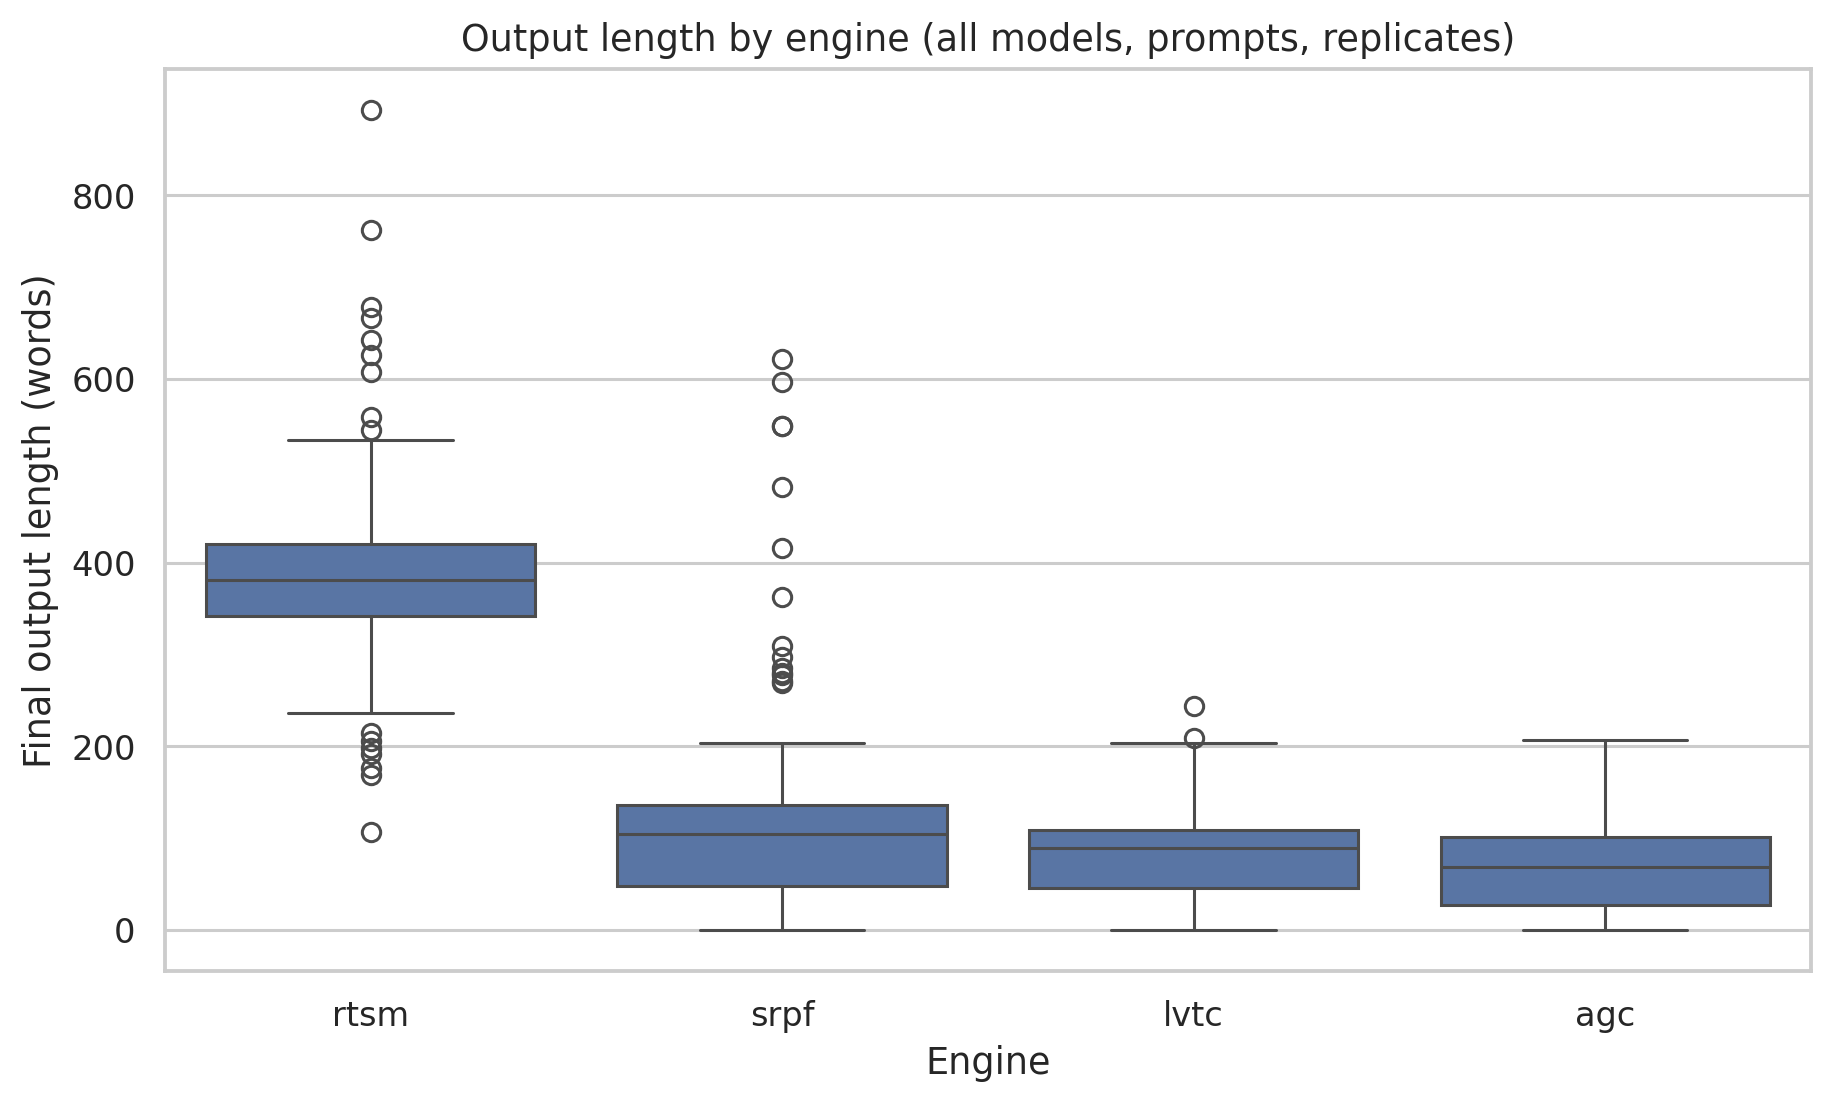
\includegraphics[width=0.72\linewidth]{figures/fig_engine_output_length_boxplot.png}
\caption{Output length differs strongly by engine, with RTSM producing substantially longer continuations than the other methods.}
\label{fig:engine_length}
\end{figure}

\begin{figure}[t]
\centering
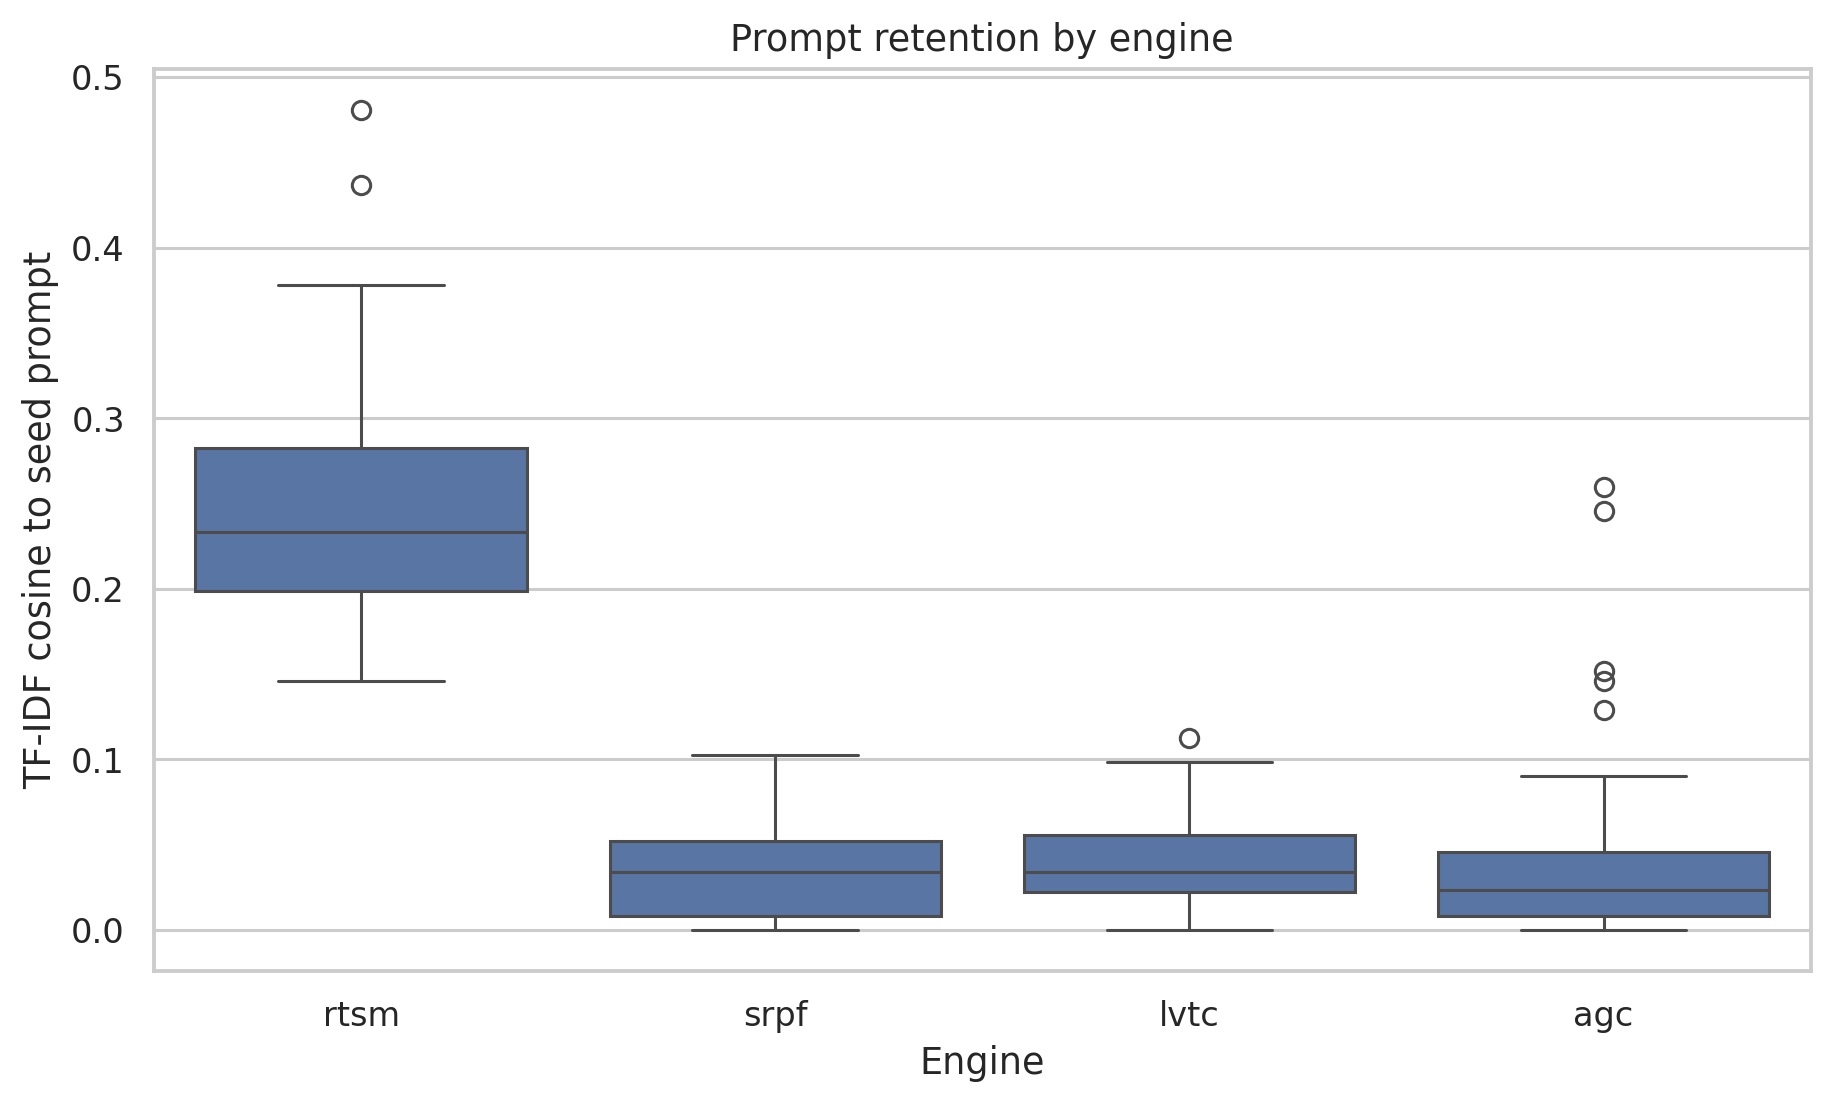
\includegraphics[width=0.72\linewidth]{figures/fig_engine_prompt_similarity_boxplot.png}
\caption{Prompt retention by engine. RTSM preserves markedly more lexical alignment to the seed prompt than AGC, LVTC, or SRPF.}
\label{fig:engine_prompt_similarity}
\end{figure}

\begin{figure}[t]
\centering
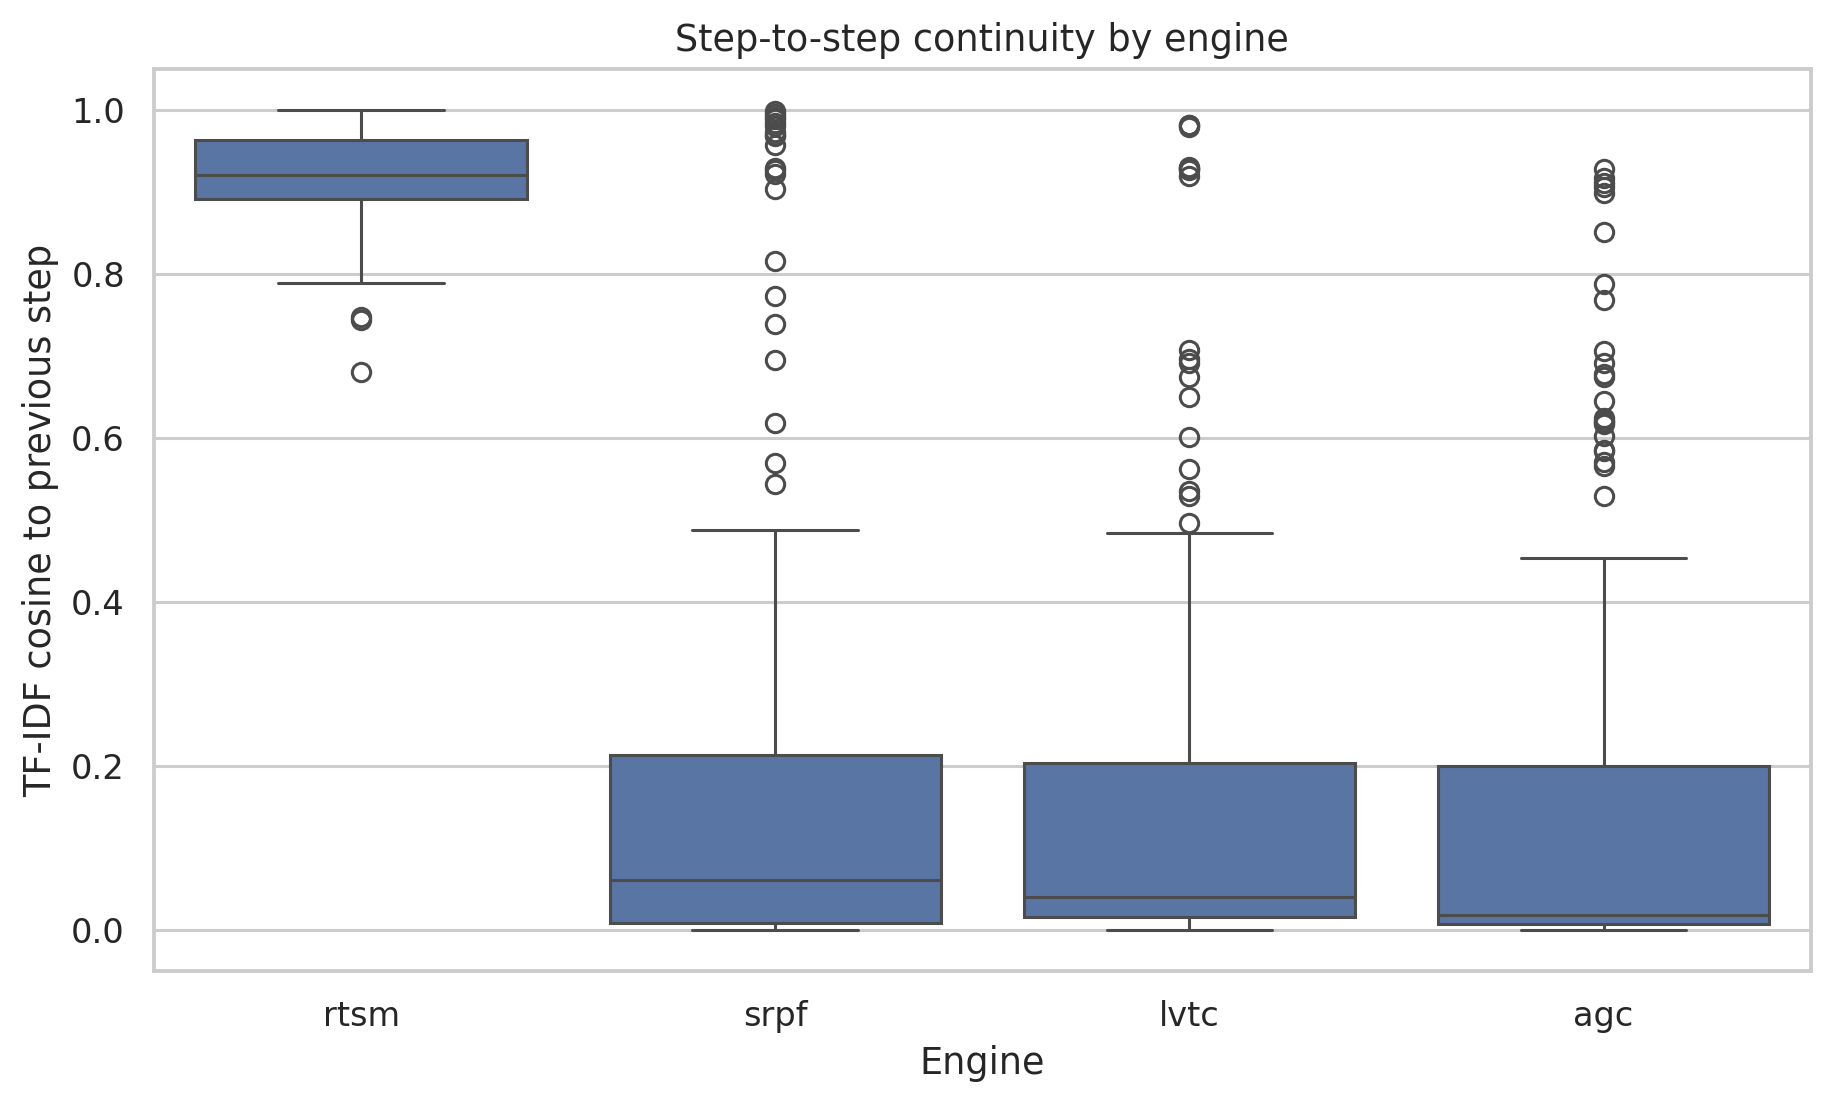
\includegraphics[width=0.72\linewidth]{figures/fig_engine_previous_step_similarity_boxplot.png}
\caption{Step-to-step continuity by engine. RTSM remains close to the previous step, while AGC, LVTC, and SRPF drift more between recursive iterations.}
\label{fig:engine_prev_similarity}
\end{figure}

\begin{figure}[t]
\centering
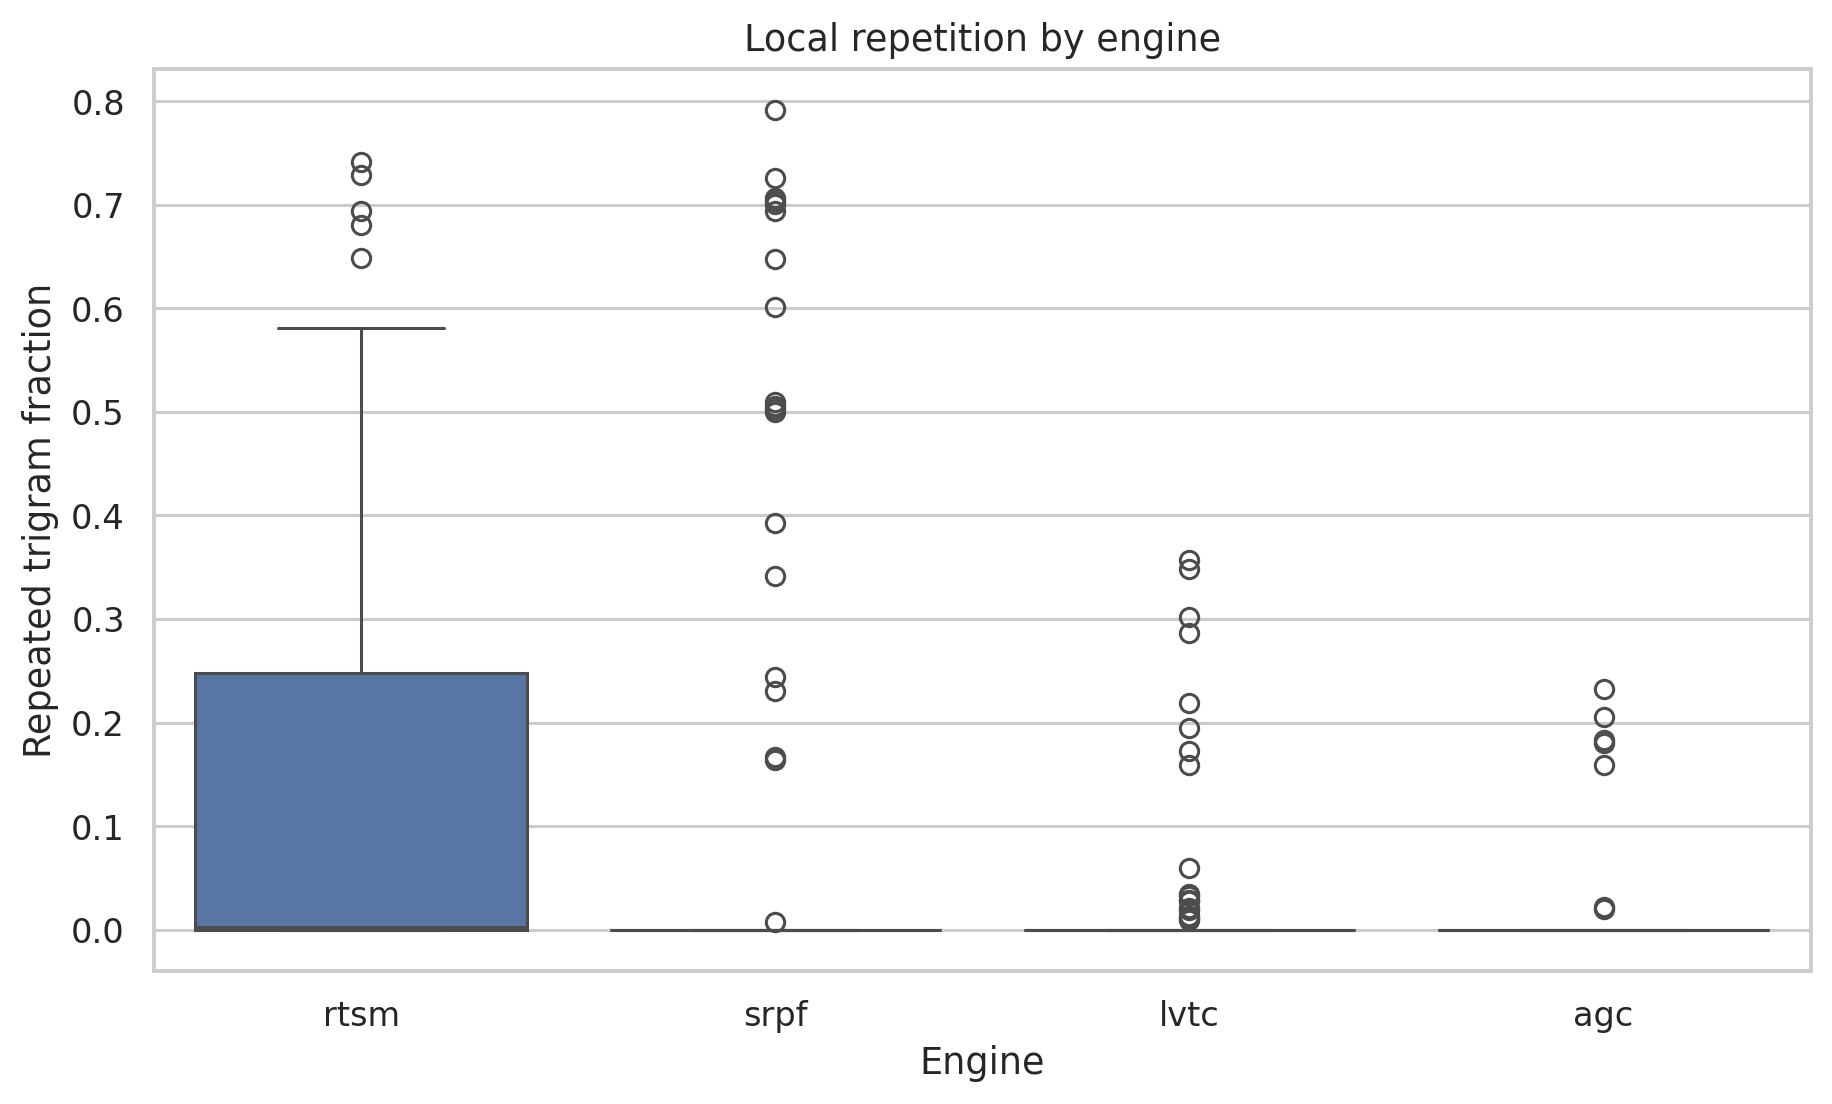
\includegraphics[width=0.72\linewidth]{figures/fig_engine_repetition_boxplot.png}
\caption{Repetition cost of persistence. RTSM and SRPF show materially higher repeated trigram fractions than AGC or LVTC.}
\label{fig:engine_repetition}
\end{figure}

\begin{figure}[t]
\centering
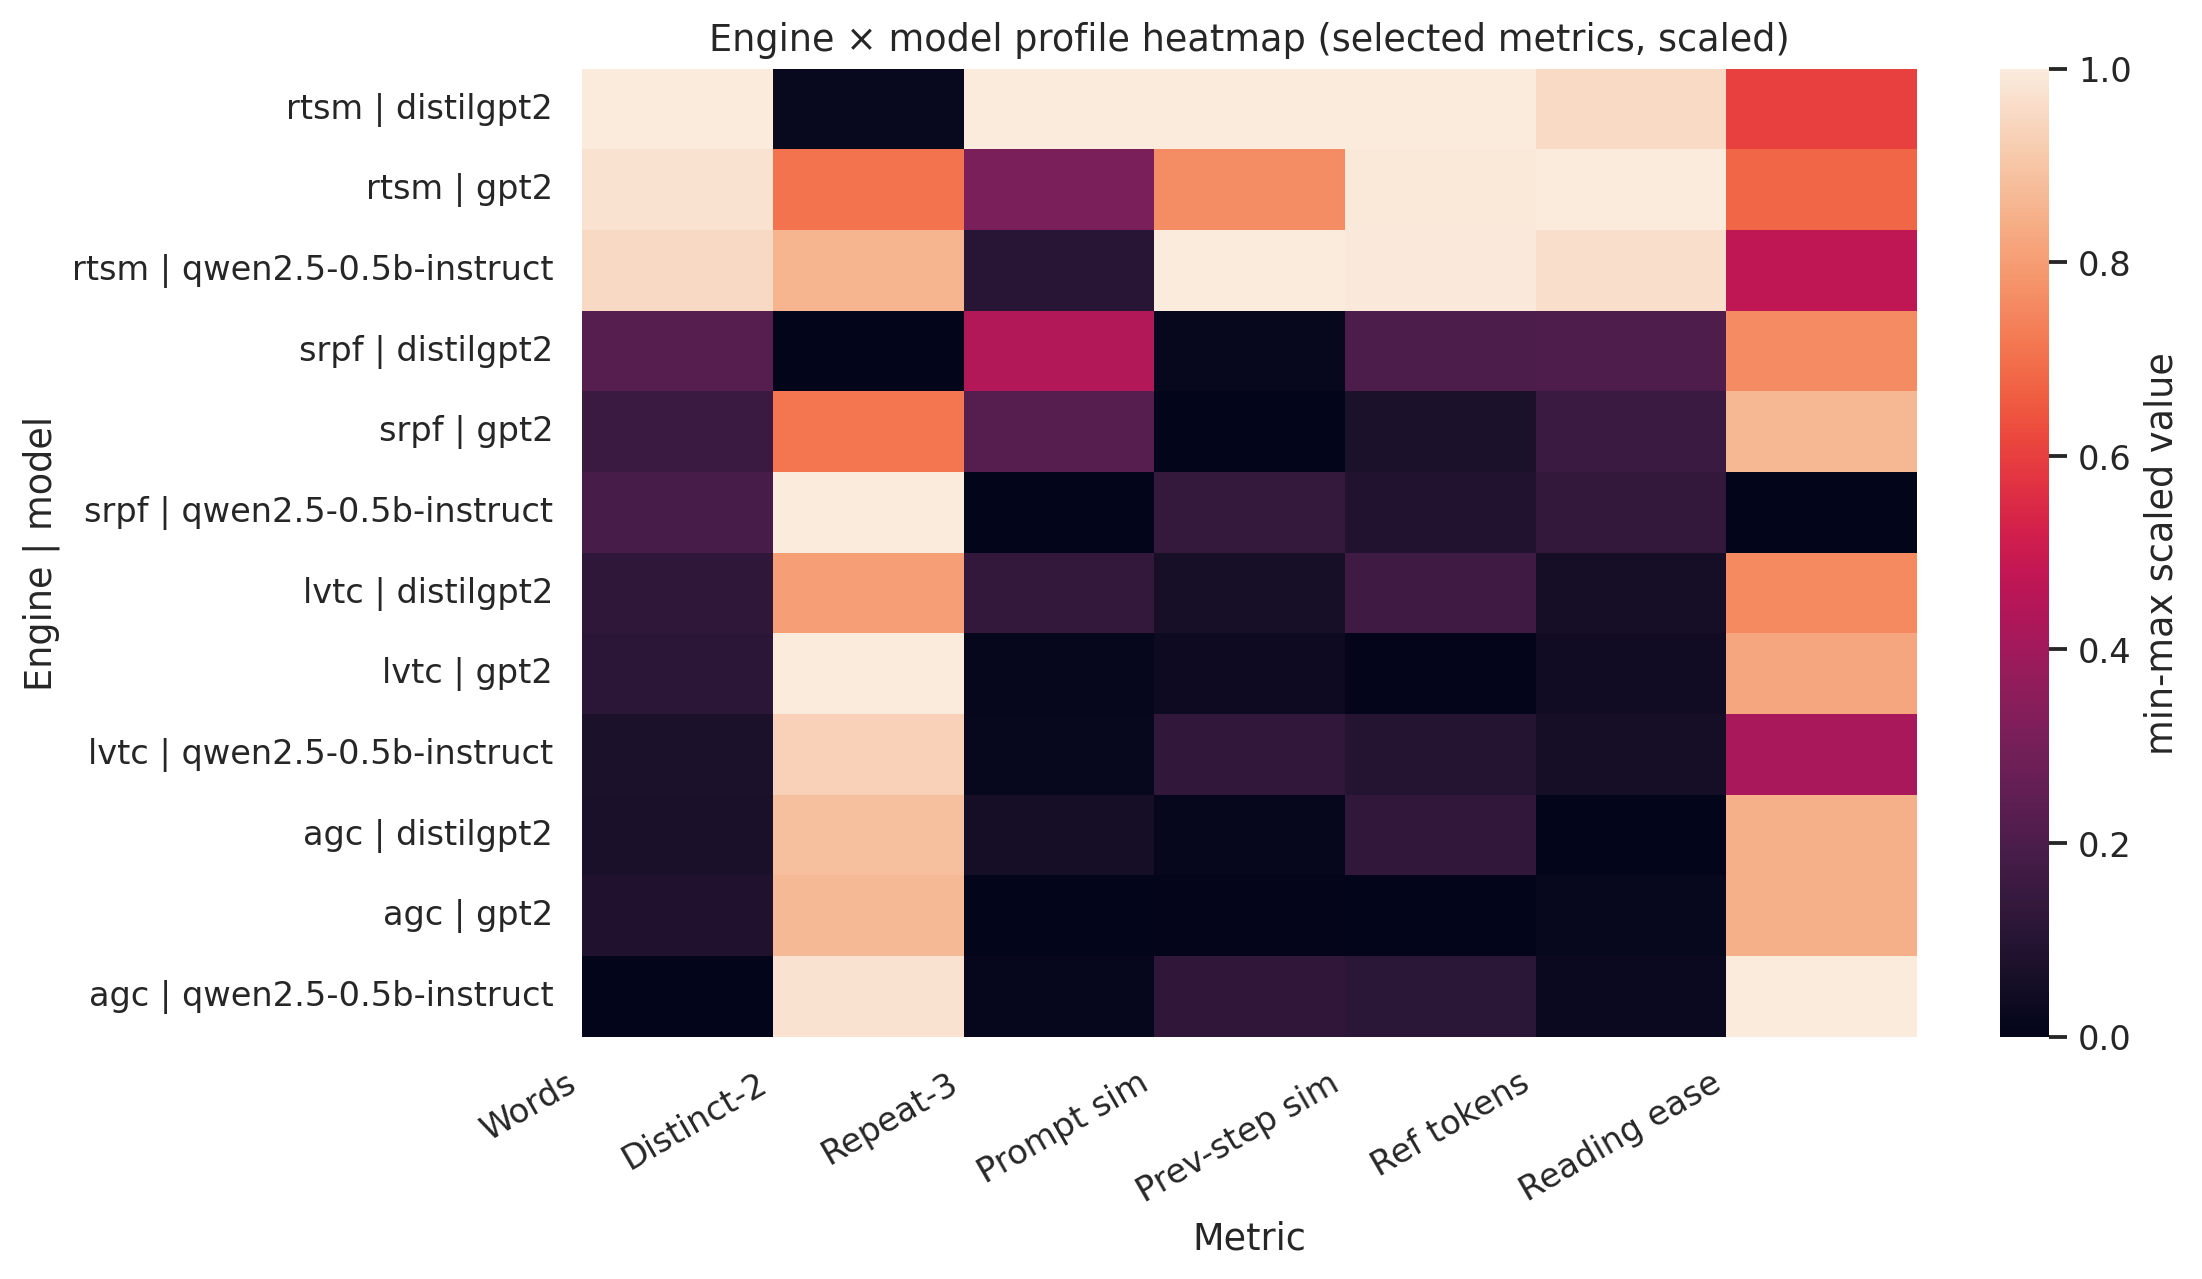
\includegraphics[width=0.90\linewidth]{figures/fig_engine_model_profile_heatmap.png}
\caption{Engine--model profile heatmap for selected metrics after min--max scaling within each metric.}
\label{fig:engine_model_heatmap}
\end{figure}

\begin{figure}[t]
\centering
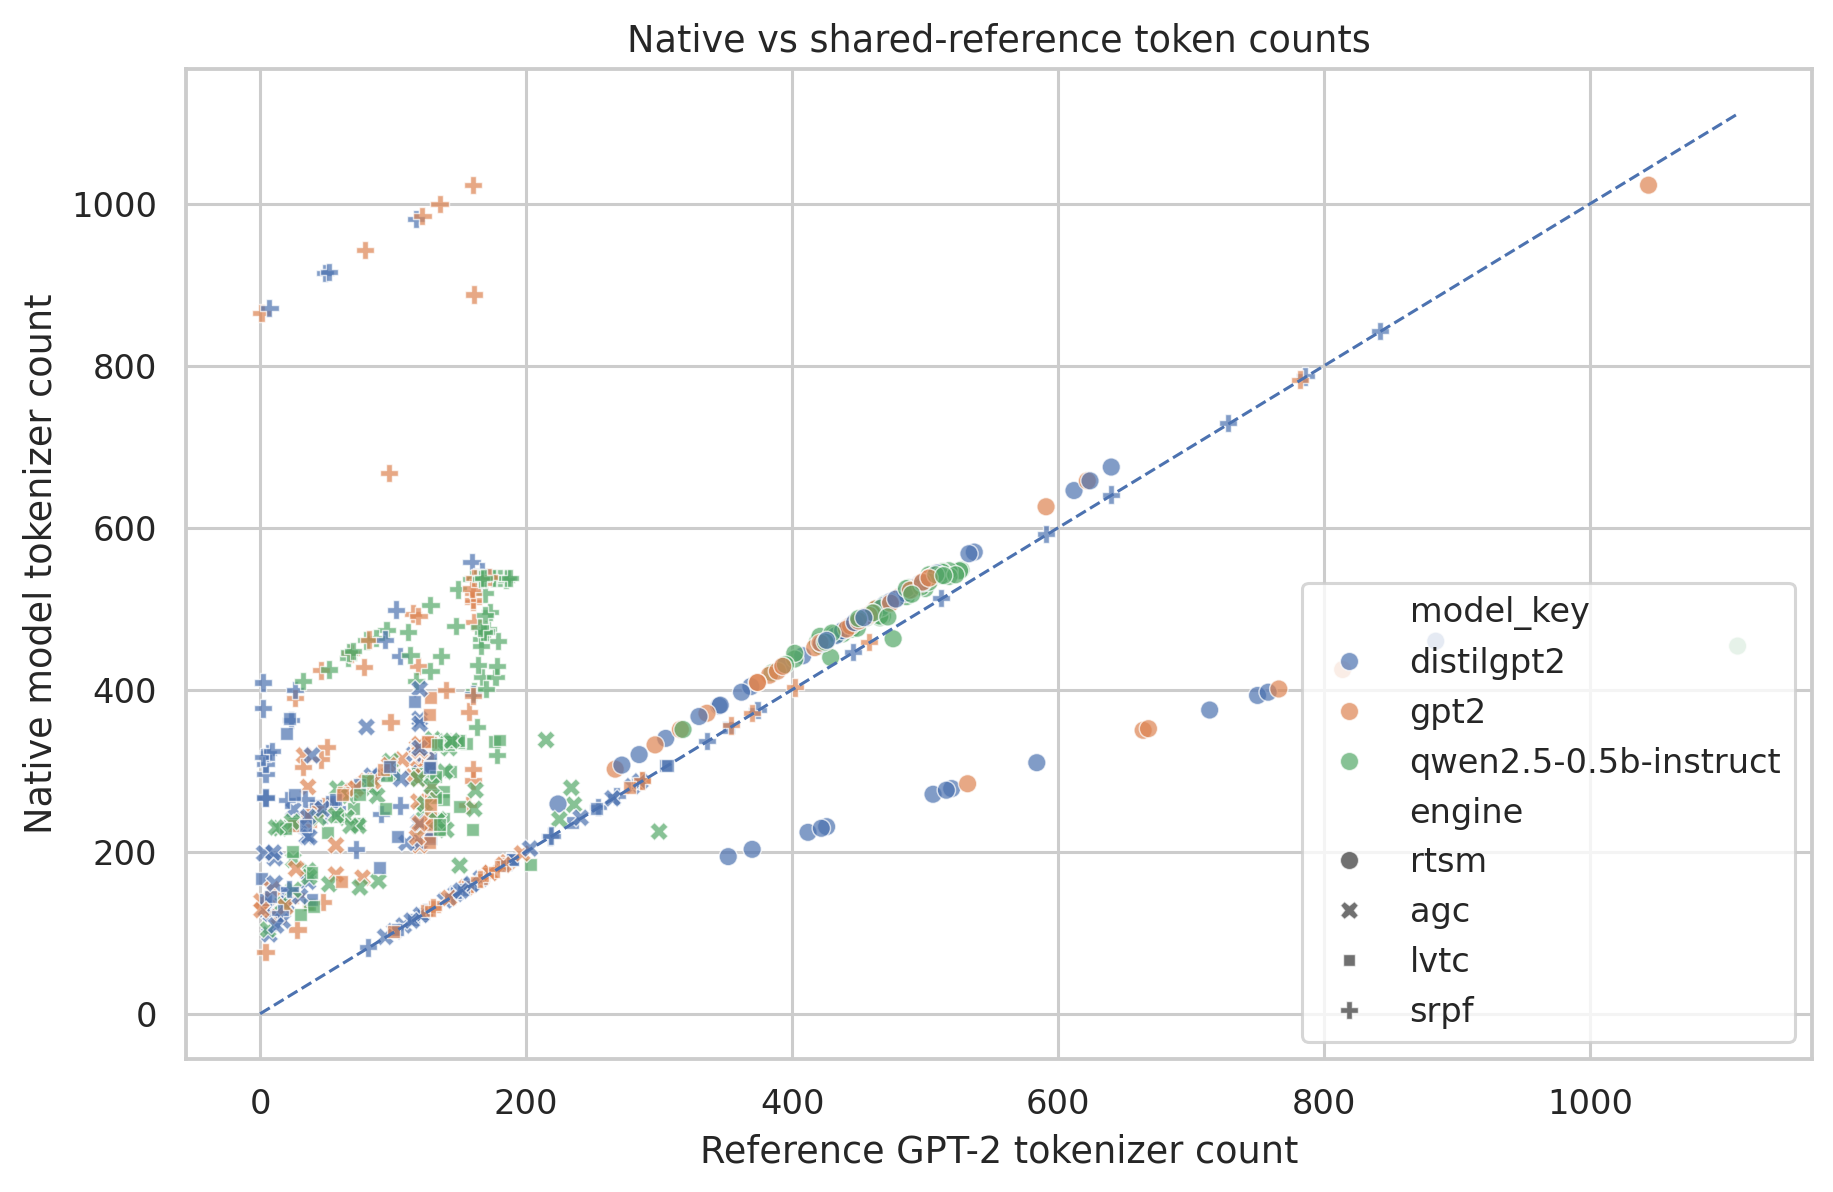
\includegraphics[width=0.78\linewidth]{figures/fig_native_vs_reference_tokens_scatter.png}
\caption{Native tokenizer counts versus shared-reference tokenizer counts. Native counts vary strongly by model; reference counts provide a more stable basis for cross-model comparison.}
\label{fig:native_vs_reference_tokens}
\end{figure}

\begin{figure}[t]
\centering
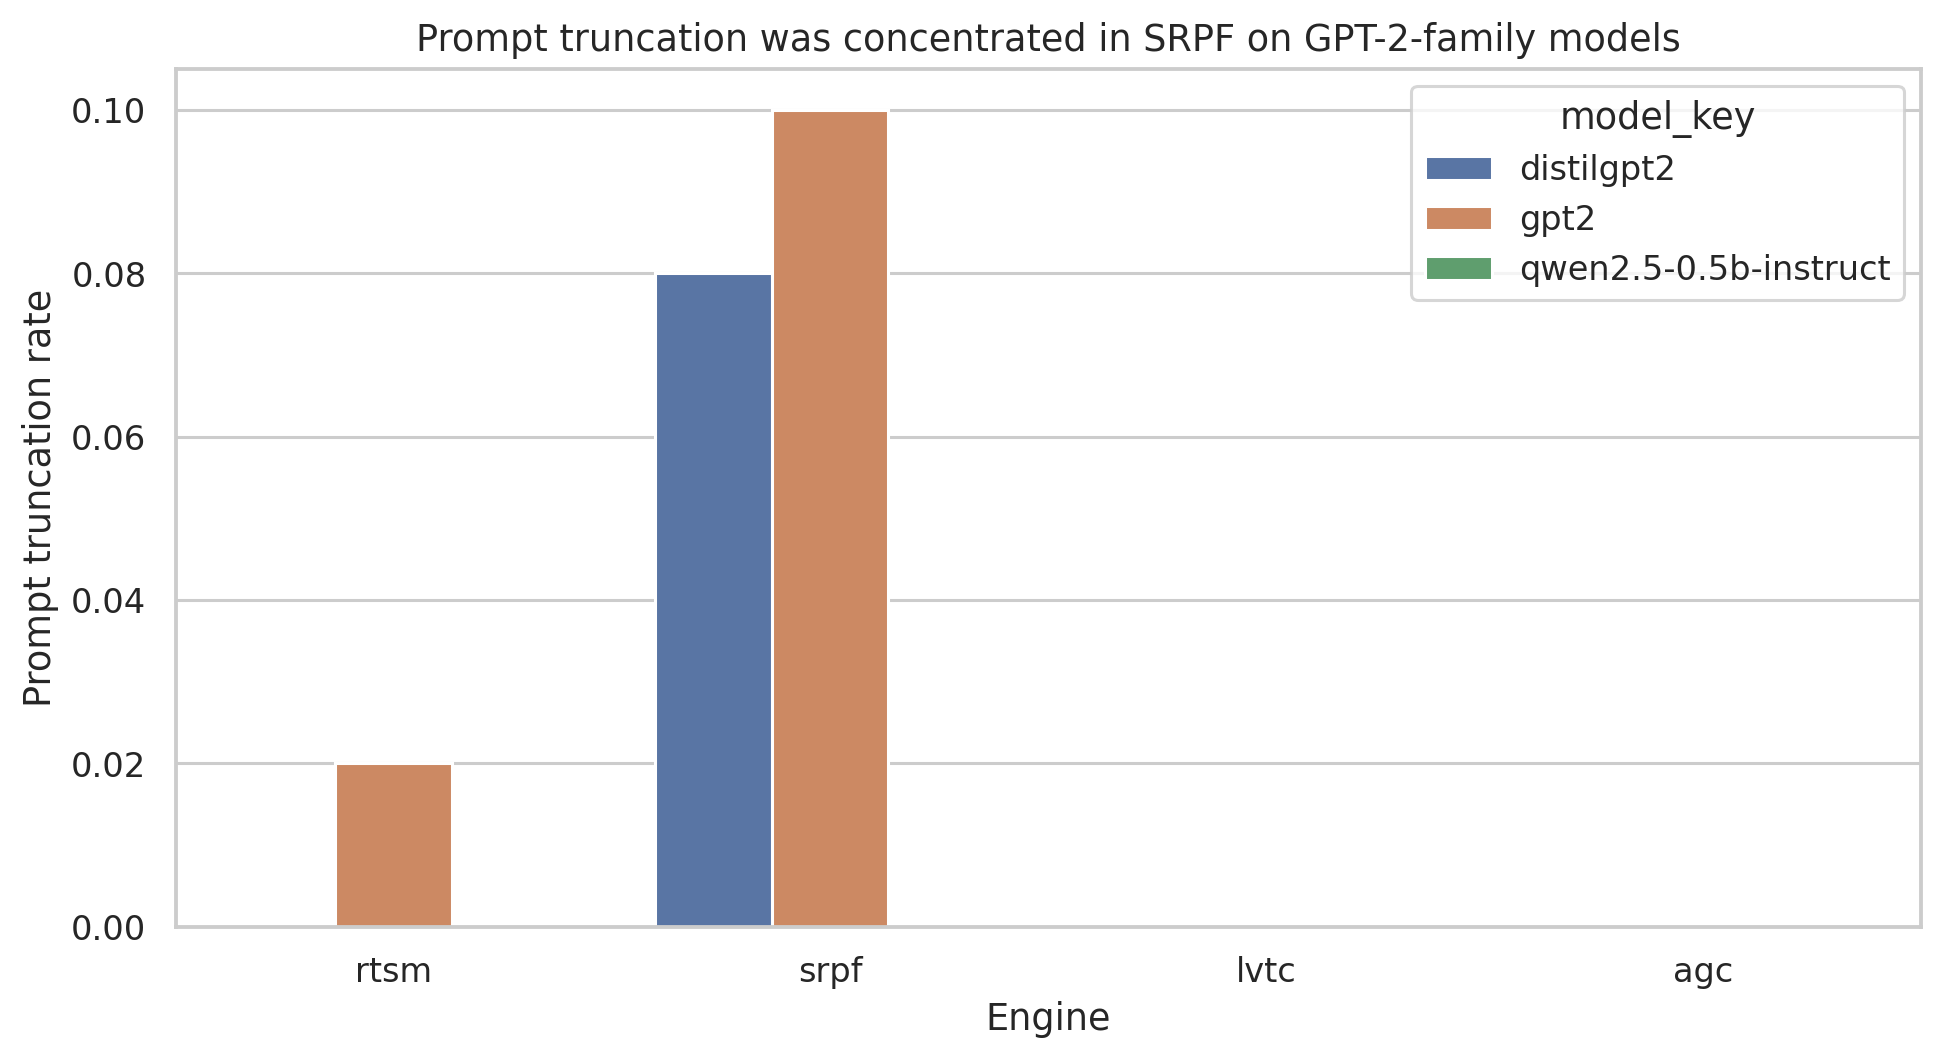
\includegraphics[width=0.75\linewidth]{figures/fig_truncation_rate_bar.png}
\caption{Prompt truncation was concentrated in SRPF on the GPT-2-family models, reflecting its tendency to grow the recursive prompt.}
\label{fig:truncation_rate}
\end{figure}
